\documentclass{article}
% Change "article" to "report" to get rid of page number on title page
\usepackage{amsmath,amsfonts,amsthm,amssymb}
\usepackage{setspace}
\usepackage{Tabbing}
\usepackage{fancyhdr}
\usepackage{lastpage}
\usepackage{extramarks}
\usepackage{chngpage}
\usepackage{soul,color}
\usepackage{graphicx,float,wrapfig}
\usepackage{xcolor}
\usepackage{textcomp}
\usepackage{listings}

\usepackage{caption}
\DeclareCaptionFont{white}{\color{white}}
\DeclareCaptionFormat{listing}{\colorbox{gray}{\parbox{\textwidth}{#1#2#3}}}
\captionsetup[lstlisting]{format=listing,labelfont=white,textfont=white}

% In case you need to adjust margins:
\topmargin=-0.45in      %
\evensidemargin=0in     %
\oddsidemargin=0in      %
\textwidth=6.5in        %
\textheight=9.0in       %
\headsep=0.25in         %

\setlength{\parindent}{1cm}


\lstset{language=Java,tabsize=3,frame=lines,keywordstyle=\color{blue},commentstyle=\color{purple},stringstyle=\color{red},numbers=left,numberstyle=\tiny,numbersep=5pt,breaklines=true,showstringspaces=false,basicstyle=\footnotesize,emph={label}}


% Document Specific Information
\newcommand{\Title}{Succincter}
\newcommand{\Date}{Tuesday,\ December\ 11,\ 2012}
\newcommand{\Class}{Computer Science 222}
\newcommand{\ClassTime}{}
\newcommand{\ClassInstructor}{Professor Mitzenmacher}
\newcommand{\AuthorName}{Dan Bradley (dbradley@college), Saagar Deshpande (sdeshpande@college)}

% Setup the header and footer
\pagestyle{fancy}                                                       %
\lhead{Bradley, Deshpande}                                                 %
%\chead{\Class\ (\ClassInstructor\ \ClassTime): \Title}  %
\chead{\Title}  %
\rhead{\Date}                                                     %
\lfoot{\lastxmark \Class}                                                      %
\cfoot{}                                                                %
\rfoot{Page\ \thepage\ of\ \pageref{LastPage}}                          %
\renewcommand\headrulewidth{0.4pt}                                      %
\renewcommand\footrulewidth{0.4pt}                                      %

% This is used to trace down (pin point) problems
% in latexing a document:
%\tracingall


%%%%%%%%%%%%%%%%%%%%%%%%%%%%%%%%%%%%%%%%%%%%%%%%%%%%%%%%%%%%%
% Make title
\title{\textmd{\textbf{\Class:\ \Title}}\\\normalsize\vspace{0.1in}\small{ \Date}\\\vspace{0.1in}\large{\textit{\ClassInstructor\ \ClassTime}}}
\author{\textbf{\AuthorName}}
\date{Final Project}
%%%%%%%%%%%%%%%%%%%%%%%%%%%%%%%%%%%%%%%%%%%%%%%%%%%%%%%%%%%%%

\begin{document}

\maketitle

\bigskip
\centerline{**********}

\noindent \section{Abstract}
Using Mihai Patrascu's 2008 paper "Succincter",  we implement a way to store trits (trinary values) within 1.05\% of the ideal space of $n*log_2(3)$ while having lookup in $O(t)$ time, where $t$ is the depth of our data structure. We find that this is both a fast and space efficient data structure with room for extension past simply storing trits.

\noindent \section{Introduction}

There are few effective methods for storing trits


\centerline{**********}

\noindent \section{Implementation}


\bigskip

\noindent \section{Results and Analysis}

\begin{figure}[htb]
\centering
\begin{minipage}{.5\textwidth}
  \centering
  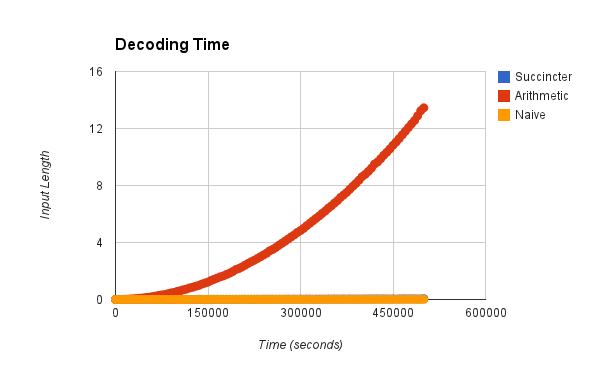
\includegraphics[scale=0.4]{images/decoding_time}
  \captionof{figure}{A figure}
  \label{fig:test1}
\end{minipage}%
\begin{minipage}{.5\textwidth}
  \centering
  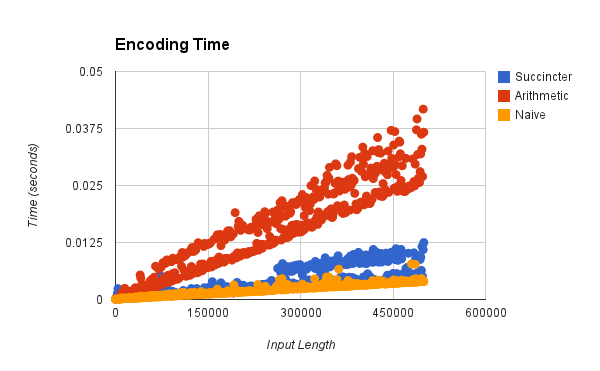
\includegraphics[scale=0.4]{images/encoding_time}
  \captionof{figure}{Another figure}
  \label{fig:test2}
\end{minipage}
\end{figure}


\bigskip

\noindent \section*{Conclusion}

\bigskip
\centerline{**********}


\noindent \section*{Appendix}

%\lstinputlisting[language=java,label=problem4,caption=Code for Problem 4]{pset4problem4.java}

%\lstinputlisting[language=java,label=problem5,caption=Code for Problem 5]{countmin.java}

%\begin{lstlisting}[language=java,label=some-code,caption=Some Code]
% Connection db = DriverManager.getConnection("jdbc:h2:rel.db", "user", "pass");
%  Statement stmt = db.createStatement();
%  stmt.execupdate("INSERT INTO CAMPAIGN VALUES ('C1R1R2R3R4R5R6', 1234, 1170, 1189, 1934)");
%\end{lstlisting}
\end{document}

%%%%%%%%%%%%%%%%%%%%%%%%%%%%%%%%%%%%%%%%%%%%%%%%%%%%%%%%%%%%%

